%%*****************************************************************************
%% $Id$
%%*****************************************************************************
%% Author: Gerd Neugebauer
%%-----------------------------------------------------------------------------
\documentclass[12pt,div12,a4paper]{scrbook}

\usepackage[latin1]{inputenc}
\usepackage{booktabs}
\usepackage{listings}
\usepackage{graphicx,color}

\definecolor{hellmagenta}{rgb}{1,0.75,0.9}
\definecolor{hellcyan}{rgb}{0.75,1,0.9}
\definecolor{hellgelb}{rgb}{1,1,0.8}
\definecolor{backgroundColor}{rgb}{1,1,0.8}
\definecolor{colKeys}{rgb}{0,0,.8}
\definecolor{colIdentifier}{rgb}{0,0,0}
\definecolor{colComments}{rgb}{.7,.2,.2}
\definecolor{colString}{rgb}{0,0.5,0}
\definecolor{darkyellow}{rgb}{1,0.9,0}
%
\usepackage{listings}
\lstset{%
    language=[AlLaTeX]TEX,%
    float=hbp,%
    basicstyle=\ttfamily\small, %
    identifierstyle=\color{colIdentifier}, %
    keywordstyle=\color{colKeys}\bf\tt, %
    stringstyle=\color{colString}, %
    commentstyle=\color{colComments}, %
    columns=flexible, %
    tabsize=3, %
    frame=single, %
    extendedchars=true, %
    showspaces=false, %
    showstringspaces=false, %
    numbers=none,% left, %
    numberstyle=\tiny\sf, %
    breaklines=true, %
    backgroundcolor=\color{backgroundColor}, %
    breakautoindent=true, %
    captionpos=b,%
    xleftmargin=\fboxsep,%
    xrightmargin=\fboxsep%
}
%\usepackage[colorlinks]{hyperref}
%

\lstset{%
    language=[LaTeX]TEX,%
    float=hbp,%
    basicstyle=\ttfamily\small, %
    identifierstyle=\color{colIdentifier}, %
    keywordstyle=\color{colKeys}\bf\tt, %
    stringstyle=\color{colString}, %
    commentstyle=\color{colComments}, %
    columns=flexible, %
    tabsize=4, %
    frame=single, %
    extendedchars=true, %
    showspaces=false, %
    showstringspaces=false, %
    numbers=none,% =left, %
    numberstyle=\tiny\sf, %
    breaklines=true, %
    backgroundcolor=\color{backgroundColor}, %
    breakautoindent=true, %
    captionpos=b,%
    xleftmargin=\fboxsep,%
    xrightmargin=\fboxsep%
}
\lstset{%
    language=Java,%
    float=hbp,%
    basicstyle=\ttfamily\small, %
    identifierstyle=\color{colIdentifier}, %
    keywordstyle=\color{colKeys}\bf\tt, %
    stringstyle=\color{colString}, %
    commentstyle=\color{colComments}, %
    columns=flexible, %
    tabsize=4, %
    frame=single, %
    extendedchars=true, %
    showspaces=false, %
    showstringspaces=false, %
    numbers=none,% =left, %
    numberstyle=\tiny\sf, %
    breaklines=true, %
    backgroundcolor=\color{backgroundColor}, %
    breakautoindent=true, %
    captionpos=b,%
    xleftmargin=\fboxsep,%
    xrightmargin=\fboxsep%
}

\usepackage[colorlinks=true]{hyperref}

\providecommand*{\ExTeX}{\ifx\texorpdfstring\undefined
  \textrm{% the logo comes always with serifs
    \ensuremath{\textstyle\varepsilon_{\kern-0.15em\mathcal{X}}}%
    \kern-.15em\TeX}%
  \else\texorpdfstring{%
  \textrm{% the logo comes always with serifs
    \ensuremath{\textstyle\varepsilon_{\kern-0.15em\mathcal{X}}}%
    \kern-.15em\TeX
  }}{ExTeX}%
  \fi
}

\newcommand\INCOMPLETE{\bigskip\par{\unitlength=1mm\framebox(60,20){To be completed.}}\bigskip\par}

\newenvironment{abstract}{\begin{quotation}}{\end{quotation}}

\title{ExTeX User's Guide}
\author{Gerd Neugebauer}
%\date{}

\begin{document}%%%%%%%%%%%%%%%%%%%%%%%%%%%%%%%%%%%%%%%%%%%%%%%%%%%%%%%%%%%%%%%

\begin{titlepage}
  \begin{center}
  \vspace*{1pt}
  \vfill
  
\includegraphics[width=\textwidth]{ExTeX-splash.png}
  \vfill
  \textsf{\Huge User's Guide}
  \vfill
  \textsf{\Large Version 0.1}
  \vfill
  \textsf{\large Gerd Neugebauer}
  \vfill
  \vfill
%\maketitle

  \begin{abstract}
    This document describes some basic steps to develop and test \ExTeX.
    It is meant for newcomers to the project or people who want to
    evaluate \ExTeX.
  \end{abstract}
  \end{center}
\newpage
\footnotesize
\copyright\ 2005 The \ExTeX\ Group and individual authors listed below 

\ExTeX{} is free software; you can redistribute it and/or modify it
under the terms of the \href{LGPL.html}{LibraryGNU General Public
  License} as published by the Free Software Foundation; either
version 1, or (at your option) any later version.

\ExTeX{} is distributed in the hope that it will be useful, but
WITHOUT ANY WARRANTY; without even the implied warranty of
MERCHANTABILITY or FITNESS FOR A PARTICULAR PURPOSE.  See the
\href{LGPL.html}{Library GNU General Public License} for more details.

You should have received a copy of the \href{LGPL.html}{Library GNU
  General Public License} along with this documentation; see the file
\href{LGPL.html}{LICENSE.txt}.  If not, write to the Free Software
Foundation, 675 Mass Ave, Cambridge, MA 02139, USA. 
\vfill

\noindent
Gerd Neugebauer\\
Im Lerchelsb\"ohl 5\\
64521 Gro\ss-Gerau (Germany)\smallskip\par\noindent WWW:
\url{http://www.gerd-neugebauer.de/}
\smallskip\par\noindent Net: \href{mailto://gene@gerd-neugebauer.de}{gene@gerd-neugebauer.de}

\end{titlepage}


\newpage
\tableofcontents
\newpage

\chapter{Introduction}
%@author Gerd Neugebauer

\ExTeX{} aims at providing a high-quality typesetting system. The
development of \ExTeX\ has been inspired by the experiences with \TeX.
The focus lies on an open design and a high degree of configurability.
Thus \ExTeX\ should be a good base for further development.

On the other hand we have to take care not to leave the current user
base of \TeX\ behind. pdf\TeX\ has taught us that a migration path
from \TeX\ has a positive value in it. In the mean time the majority
of \TeX\ users applies in fact pdf\TeX.

To provide a backward compatibility of \ExTeX\ with \TeX\ one special
configuration is provided. Thus backward compatibility is just a
matter of configuration.


\section{Web Site}
%@author Gerd Neugebauer

There is a web site devoted to \ExTeX. This web site can be reached
via the URL

\begin{quotation}
  \url{http://www.extex.org}
\end{quotation}


\section{Mailing Lists}
%@author Gerd Neugebauer

If you are ready to try \ExTeX{} you might as well want to join a
mailing list to get in contact with the community.

\begin{quotation}
  \url{http://www.dante.de/listman/extex}
\end{quotation}


\chapter{Getting Started}
%@author Gerd Neugebauer

In this chapter we describe the steps you can take to get \ExTeX\ up
and running. We try to use as few as possible premises. Thus it should
be not too hard to get started.

\section{Prerequisites}
%@author Gerd Neugebauer

\subsection{Java}
%@author Gerd Neugebauer

You need to have Java 1.4.2 or later installed on your system. You can
get Java for a several systems directly from \url{java.sun.com}.
Download and install it accoring to the installation instructions for
your environment.

To check that you have an appropriate Java on your path you can use
the command \texttt{java} with the argument \texttt{-version}. This
can be seen in the following listing:

\begin{lstlisting}{}
> java -version
java version "1.4.2_06"
Java(TM) 2 Runtime Environment, Standard Edition (build 1.4.2_06-b03)
Java HotSpot(TM) Client VM (build 1.4.2_06-b03, mixed mode)
>
\end{lstlisting}


\subsection{TEXMF}
%@author Gerd Neugebauer

If you want to use more than the pure \TeX\ engine fonts and macros
can be inherited from a texmf tree. \ExTeX\ itself does not contain a
full texmf tree. It comes just with some rudimentray files necessary
for testing. Thus you should have installed a texmf tree, e.g. from a
\TeX Live installation. This can be found on the
\href{http://www.ctan.org}{Comprehensive \TeX\ Archive Network (CTAN)}.

There is no need to install the texmf tree in a special place. You
have to tell \ExTeX\ anyhow where it can be found. It is even possible
to work with several texmf trees.

One requirement for the texmf trees is that they have a file database
(\texttt{ls-R}). \ExTeX\ can be configured to work without it, but
then \ExTeX\ is deadly slow. Thus you do not really want to try this
alternative.


\section{Getting \ExTeX}
%@author Gerd Neugebauer

\subsection{Getting the Sources}
%@author Gerd Neugebauer

The sources of \ExTeX\ are stored in a RCS repository. To access this
repository you need access to the internet and RCS installed in some
way.

The coordinates of the repository are:
\medskip

\begin{tabular}{ll}\toprule
  Connection type: & \texttt{pserver}			\\
  User:		   & \texttt{anonymous}			\\
  Host:		   & \texttt{cvs.extex.berlios.de}	\\
  Location:	   & \texttt{/cvsroot/extex}		\\
  Module:	   & \texttt{ExTeX}			\\\bottomrule
\end{tabular}
\bigskip

We assume here that you have access to cvs on the command line. This
can be either a shell on a Unix-like system or somethng like cygwin on
Windows. We also assume that you have direct connection to the internet.

First we create a directory where the sources are stored:
\begin{lstlisting}{}
> mkdir ExTeX
\end{lstlisting}

Next we change the current directory to this base directory:
\begin{lstlisting}{}
> cd ExTeX
\end{lstlisting}

Now we log into the CVS repository. This login uses an anonymous
account. This enables us to download the sources but not to commit any
changes. The committing is restricted to members of the \ExTeX{} team.
\begin{lstlisting}{}
> cvs -d:pserver:anonymous@cvs.extex.berlios.de/cvsroot/extex login
\end{lstlisting}

Finally we can check out the sources:
\begin{lstlisting}{}
> cvs -d:pserver:anonymous@cvs.extex.berlios.de/cvsroot/extex co ExTeX
\end{lstlisting}

This command shows a lot of output. At the end the current directory
is filled with a lot of files and directories.

\section{Installing \ExTeX}
%@author Gerd Neugebauer

\subsection{Installing \ExTeX\ with the Installer}\label{sec:installer}
%@author Gerd Neugebauer

\begin{figure}[tp]
  \centering
  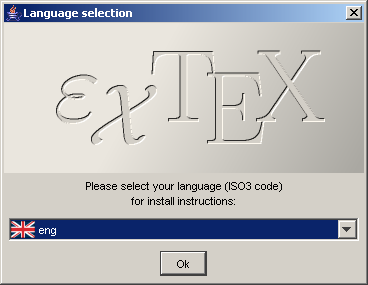
\includegraphics[width=.8\textwidth]{inst1.png}
  \caption{The Language Selection in the Installer}
  \label{fig:inst1}
\end{figure}
The easiest installation of \ExTeX\ works with the \ExTeX\ installer.
This installer is named \texttt{ExTeX-setup.jar}. You can start the
installer with the following command line:

\begin{lstlisting}{}
> java -jar ExTeX-setup.jar
\end{lstlisting}

On windows with a properly installed Java you can also start the
installer by double-clicking \texttt{ExTeX-setup.jar} in the Explorer.

The installer provides a graphical user interface with a wizard
guiding you through the installation process. The first dialog is
shown in figure~\ref{fig:inst1}. As you can see you can select one of
several languages for the installation process. Currently the
languages English and German are supported. There might be some more
at the time you are performing the installation.

Note that the internationalization covers the installer only. \ExTeX\
can be run under different language environments as well. This is
controlled by a setting at run-time. Currently only an English
language binding for \ExTeX\ is provided.

Finally you have to make sure that the executables \texttt{extex} or
\texttt{extex.bat} is on your path for executables.


\subsection{Replaying an Installation}
%@author Gerd Neugebauer

Sometimes it is desirable to perform an installation on several
similar machines. This means that the answers to the questions in the
installer are the same. This process can be automated.
\begin{figure}[tp]
  \centering
  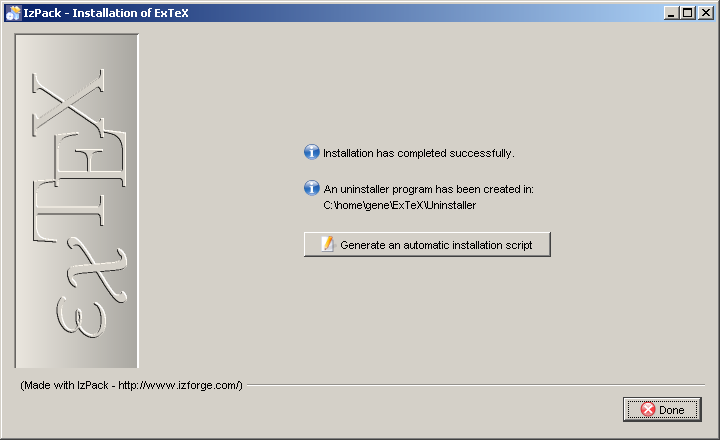
\includegraphics[width=.8\textwidth]{inst8.png}
  \caption{Generating a Auto-Configuration for the Installer}
  \label{fig:inst8}
\end{figure}

In figure~\ref{fig:inst8} you can see the last screen of the
installer. Here you have the possibility to select the button
``Generate an automatic installation script''. This produces an XML
file which can be passed to the installer to avoid the dialogs.

Suppose you have named the file \texttt{replay.xml} in the file
selector which pops up when the button has been pressed. Then you can
replay the installation with the following command invocation:

\begin{lstlisting}{}
> java -jar ExTeX-setup.jar replay.xml
\end{lstlisting}

This supposes that the two files \texttt{ExTeX-setup.jar} and
\texttt{replay.xml} are in the current directory.

Finally you have to make sure that the executables \texttt{extex} or
\texttt{extex.bat} is on your path for executables.


\subsection{Creating the \ExTeX\ Installer}
%@author Gerd Neugebauer

You can create the installer of \ExTeX\ from the sources. All you need
for this step is contained in the source distribution. Suppose you are
in the base directory of the distribution. Then the following command
creates the installer:

\begin{lstlisting}{}
> build installer
\end{lstlisting}

As a result the file \texttt{ExTeX-setup.jar} is created in the
directory \texttt{target}. This file is a self-contained installer.
You can immediately start the installer with the following command line:

\begin{lstlisting}{}
> java -jar target/ExTeX-setup.jar
\end{lstlisting}

In addition the installer file can be moved to any other place -- even
other machines -- and run the installation there (see also
section~\ref{sec:installer}).


\subsection{Installing \ExTeX\ from the Sources on the Command Line}
%@author Gerd Neugebauer

To install you can use the build script provided in the \ExTeX{}
base directory.

\begin{lstlisting}{}
> build -Dinstall.dir=/usr/local/share/ExTeX install
\end{lstlisting}

Additionally you have to copy the file \texttt{.extex} from the base
directory of the \ExTeX\ to your home directory and adapted to your
installation. Especially the value of \texttt{extex.texinputs} most
probably needs adaption to point to your texmf trees.

Finally you have to make sure that the executables \texttt{extex} or
\texttt{extex.bat} is on your path for executables.

Now you can forget the source directory. It is not needed any more
unless you are debugging or developing \ExTeX{} extensions.


\chapter{Configuring \ExTeX}
%@author Gerd Neugebauer

The behaviour of \ExTeX\ can be influenced via command line arguments
and configuration files. Most of the times the startup files will be
enough for the casual user.


\section{Startup Files}
%@author Gerd Neugebauer

Whenever \ExTeX\ starts it looks for startup files named
\texttt{.extex}. This file is sought in the user's home directory in
in the current directory. The settings in the current directoy
overwrite the settings from the user's home directory. Those in turn
overwrite the built-in settings.

\INCOMPLETE

\section{Configuration Files}
%@author Gerd Neugebauer

Configuration files of another kind contain the assembly instructions
for \ExTeX. Those files can be used to provide additional features in
\ExTeX. 

\INCOMPLETE

\chapter{Running \ExTeX}
%@author Gerd Neugebauer

Currently \ExTeX\ can be run from the command line. In this respect it
is more or less identical to \TeX\ and can be used as a plug-in
replacement.

The following sample show a simple invocation of \ExTeX\ without any
command line arguments.

\begin{lstlisting}{}
> extex
This is ExTeX, Version 0.0 (TeX compatibility mode)
**\relax

*\end

No pages of output.
Transcript written on ./texput.log.
\end{lstlisting}

In this case \ExTeX\ enters interaction with the user and asks for an
input file. This is indicated by the two asterists. We have entered
\verb|\relax| here to indicate that we are not willing to pass in a
file name. The \ExTeX\ system asks us to enter some command --
indicted by the single asterisk. Here we have entered \verb|\end| to
indicate that we want to finish the processing. Thus \ExTeX\
terminates normally.





\INCOMPLETE

\section{Command Line Parameters}
%@author Gerd Neugebauer

\INCOMPLETE


\section{Creating Formats}
%@author Gerd Neugebauer

\INCOMPLETE


\chapter{Troubleshooting \ExTeX}
%@author Gerd Neugebauer

This chapter contains some hints in the case of trouble.

\section{Why are my files not found?}
%@author Gerd Neugebauer

\ExTeX\ has a configurable search for external resources.

\INCOMPLETE


\end{document}%%%%%%%%%%%%%%%%%%%%%%%%%%%%%%%%%%%%%%%%%%%%%%%%%%%%%%%%%%%%%%%%%
%
% Local Variables: 
% mode: latex
% TeX-master: nil
% End: 
